\documentclass[11pt,a4paper]{article}
\usepackage{iftex}
\ifPDFTeX
\usepackage[utf8]{inputenc}
\usepackage[T1]{fontenc}
\usepackage{lmodern}
\else
\usepackage{fontspec}
\setmainfont{lmroman10-regular.otf}[BoldFont=lmroman10-bold.otf,ItalicFont=lmroman10-italic.otf,BoldItalicFont=lmroman10-bolditalic.otf]
\setmonofont{lmmono10-regular.otf}
\fi
\usepackage[ngerman]{babel}
\usepackage[a4paper,margin=24mm]{geometry}
\usepackage{microtype}
\usepackage{amsmath,amssymb}
\usepackage{booktabs,longtable,tabularx,array}
\usepackage{enumitem}
\usepackage{xcolor}
\usepackage{graphicx}
\usepackage{caption}
\usepackage{xurl}
\usepackage{hyperref}

\definecolor{navy}{HTML}{12334A}
\definecolor{teal}{HTML}{146B75}
\definecolor{signal}{HTML}{A8391A}
\definecolor{softgrey}{HTML}{F1F3F5}
\hypersetup{colorlinks=true,linkcolor=navy,citecolor=teal,urlcolor=teal,
  pdftitle={Ein erstes Ranking für den S\&P 500: Monte-Carlo-Auswertung zweier Datenperioden},
  pdfauthor={ETHack 2026}}
\urlstyle{same}

\newcolumntype{P}[1]{>{\raggedright\arraybackslash}p{#1}}
\newcolumntype{R}{>{\raggedleft\arraybackslash}X}
\newcommand{\coeq}{\ensuremath{\mathrm{CO}_{2}\mathrm{e}}}
\newcommand{\tco}{\ensuremath{\mathrm{t\,CO}_{2}\mathrm{e}}}

\setlength{\parindent}{0pt}
\setlength{\parskip}{5pt}
\setlength{\tabcolsep}{4pt}
\setlength{\emergencystretch}{2em}
\setlist{itemsep=3pt,topsep=4pt,leftmargin=*}
\renewcommand{\arraystretch}{1.17}
\setcounter{tocdepth}{2}
\captionsetup{font=small,labelfont=bf,labelsep=period,skip=6pt}

\newcommand{\befund}[1]{%
  \par\vspace{2pt}\noindent\colorbox{softgrey}{%
  \begin{minipage}{\dimexpr\linewidth-2\fboxsep}\small\vspace{3pt}#1\vspace{3pt}\end{minipage}}\par\vspace{4pt}}

\title{\textcolor{navy}{Ein erstes Ranking für den S\&P~500}\\[4mm]
\large Monte-Carlo-Auswertung auf echten Daten, getrennt nach zwei Datenperioden --\\
mit einer Prüfung dessen, was am Ansatz nicht trägt}
\author{ETHack 2026 -- Umsetzungs- und Auswertungsbericht}
\date{Datenstand und Abrufe: 12.~September 2026}

\begin{document}
\maketitle

\begin{abstract}
\noindent
Gebaut wurde eine vollständige Pipeline von der Rohdatenabfrage bis zur Rangliste und darauf eine Unsicherheitsanalyse mit 1500 Methodenkombinationen. Alle Daten stammen aus frei zugänglichen Quellen und wurden am Berichtstag selbst abgerufen: Anlagenemissionen der US-Umweltbehörde, Umsätze aus SEC-XBRL, die Indexzusammensetzung mit Branchenzuordnung sowie ein kommerzieller ESG-Snapshot als Vergleichsmaßstab. Von 503 Indexmitgliedern sind 157 bewertbar. Das Ergebnis ist bewusst kein Platz, sondern ein Band: im Median 33 Perzentilpunkte breit, was rund fünf Rangplätzen entspricht. Die Rangkorrelation zur gekauften ESG-Note liegt bei $-0{,}04$ und kippt je nach Branche zwischen $-0{,}78$ und $+0{,}51$. Für die Zeit nach 2023 existieren keine freien Emissionsdaten mehr; ein Rückwärtstest zeigt, dass eine Fortschreibung die Reihenfolge grob hält ($\rho = 0{,}84$), aber 37\,\% der Firmen um mehr als zehn Perzentilpunkte verschiebt. Abschnitt~\ref{sec:schwach} listet zehn Schwachstellen des Ansatzes, Abschnitt~\ref{sec:verbesser} neun konkrete Gegenmaßnahmen mit Aufwandsschätzung.
\end{abstract}

\vspace{2mm}
\befund{\textbf{Leseschlüssel.} Jede Zahl in diesem Bericht stammt aus einem der beigelegten Auswertungsdateien und ist mit \texttt{scripts/02\_analyse.py} reproduzierbar. Wo etwas nicht gemessen werden konnte, steht das ausdrücklich da -- nicht als Auslassung.}

\tableofcontents
\newpage

\section{Was gebaut wurde}

Die Pipeline besteht aus sieben Stufen. Jede ist ein eigenes Modul, und an drei Stellen ist sie erweiterbar, ohne dass etwas anderes angefasst werden muss.

\begin{enumerate}[label=\textbf{\arabic*.}]
\item \textbf{Quellen.} Vier Konnektoren hinter einem gemeinsamen Interface \texttt{DataSource.fetch()}. Rohantworten werden als Parquet zwischengespeichert, damit die Auswertung reproduzierbar bleibt und keine API zweimal befragt wird.
\item \textbf{Entity Resolution.} Anlagen werden über das Freitextfeld \texttt{parent\_company} den Indexmitgliedern zugeordnet.
\item \textbf{Kanonischer Datensatz.} Eine Zeile je Firma und Jahr, mit Herkunft und Konfidenz an jedem Wert.
\item \textbf{Kernnote (Achse~A).} Branchenrelativ normalisiert, gewichtet, geometrisch aggregiert.
\item \textbf{Unsicherheitsanalyse.} Dieselbe Rangliste 1500-mal mit zufällig gezogenen Methodenkombinationen.
\item \textbf{Greenwashing (Achse~B).} Getrennt gerechnet, nie in die Kernnote eingerechnet.
\item \textbf{Ausgabe.} Eine versionierte JSON-Datei als Schnittstelle zur Weboberfläche.
\end{enumerate}

Die Erweiterungsnähte: eine neue Quelle ist eine Klasse mit einem Registry-Eintrag; eine neue Kennzahl ist ein Eintrag mit Richtung und Branchenrelevanz; ein neues Verfahren für Normalisierung, Gewichtung oder Aggregation wird registriert und landet ohne weiteres Zutun im Kombinationsraum der Unsicherheitsanalyse. Das ist der eigentliche Punkt der Registry-Bauweise: Wer eine Methode ergänzt, macht das Rangband ehrlicher, nicht die Rechnung aufwendiger.

\section{Datenbasis: was wirklich zu holen war}

\subsection{Geprüfter Zugang statt zitierter Verfügbarkeit}

Tabelle~\ref{tab:quellen} hält fest, was am 12.~September 2026 tatsächlich erreichbar war. Zwei der im Vorfeld genannten Quellen halten ihr Versprechen nicht.

\begin{table}[htbp]
\centering\small
\caption{Quellen, wie sie sich beim Abruf verhalten haben}
\label{tab:quellen}
\begin{tabularx}{\textwidth}{P{3.0cm} P{3.3cm} P{3.1cm} X}
\toprule
\textbf{Quelle} & \textbf{Liefert} & \textbf{Zugang} & \textbf{Was dabei auffiel} \\
\midrule
EPA GHGRP \newline (Envirofacts) & Scope~1 je US-Anlage, Feld \texttt{parent\_company} & REST, ohne Anmeldung, läuft & Reihe endet mit Berichtsjahr 2023; 65\,155 Anlagen\-Jahr-Zeilen 2018--2023 \\
SEC XBRL \newline (\texttt{frames}) & Jahresumsatz je Firma & REST, User-Agent nötig, läuft & reicht bis Geschäftsjahr 2025; 53\,492 Zeilen; fünf Umsatz-Tags nötig, weil Firmen uneinheitlich taggen \\
S\&P-500-Liste & Ticker, GICS-Sektor, Sub-Industry, CIK & frei & 503 Mitglieder; die CIK spart den Umweg über eine Namenszuordnung zur SEC \\
ESG-Snapshot & kommerzielle Risk-Ratings & frei gespiegelt & Stand 2021, 245 Firmen -- genau die Sorte eingefrorener Datensatz, die auf Kaggle kursiert \\
Climate TRACE & Anlagen weltweit & REST, läuft & Feld \texttt{Owners} kommt leer zurück, damit keine Firmenzuordnung möglich \\
SBTi & geprüfte Klimaziele & \textcolor{signal}{kein API} & \texttt{/api/companies} antwortet mit 404; nur die Dashboard-Seite \\
\bottomrule
\end{tabularx}
\end{table}

\subsection{Der Fehler, der fast im Ergebnis gelandet wäre}

Die Emissionstabelle der EPA lässt sich nicht einfach aufsummieren. Sie enthält drei Arten von Meldern, unterschieden über das Feld \texttt{sector\_type}:

\begin{itemize}
\item \textbf{E -- Direktemittent.} Was die Anlage selbst ausstößt. Das ist Scope~1.
\item \textbf{S -- Lieferant.} Der Kohlenstoff in verkauften Kraftstoffen, der \emph{später beim Kunden} freigesetzt wird.
\item \textbf{I -- CO\textsubscript{2}-Injektion.} Eingelagertes, nicht ausgestoßenes CO\textsubscript{2}.
\end{itemize}

Eine naive Summe über alle Zeilen ergibt für 2023 rund 7\,364~Mio.~\tco. Nach Trennung bleiben \textbf{2\,578~Mio.~\tco{} echte Scope-1-Emissionen}; 4\,667~Mio.~\tco{} entfallen auf gelieferte Mengen und 119~Mio.~\tco{} auf biogenes CO\textsubscript{2}, das nach GHG-Protokoll getrennt auszuweisen und nicht in die Bruttobilanz einzurechnen ist.

\befund{\textbf{Warum das mehr ist als ein Rechenfehler.} Wer die Lieferantenzeilen mitzählt, rechnet einem Ölkonzern die Emissionen seiner Kunden als eigene an -- und zählt dieselbe Tonne ein zweites Mal bei dem Kraftwerk, das den Kraftstoff verbrennt. Das ist exakt die Doppelzählung, die das GHG-Protokoll untersagt. Der Faktor beträgt hier fast drei. Ein Ranking auf dieser Grundlage hätte die Raffineriebetreiber an das Ende jeder Liste gesetzt und dabei plausibel ausgesehen.}

\subsection{Entity Resolution: Ergebnis und Preis}

Das Feld \texttt{parent\_company} ist Freitext mit Beteiligungsquoten, im Original etwa:

\begin{quote}\footnotesize\ttfamily\raggedright
Empeco IV, LLC and USPF II Ferndale Holdings, LLC (74.33298\%);\\
Diamond Generating Corporation (14.00002\%);\\
Tenaska Energy, Inc. and Tenaska Energy Holdings, LLC (11.667\%)
\end{quote}

Der Parser zerlegt den String in Eigentümer und Anteil, normalisiert Rechtsformzusätze weg und ordnet in vier Stufen zu: exakt, über eine handgepflegte Tochter-Konzern-Tabelle, über deren Präfixe, und unscharf ab einem Schwellenwert von 92. Die Beteiligungsquote wird angerechnet -- eine zu 74\,\% gehaltene Anlage zählt ihrem Eigentümer auch nur zu 74\,\% (Equity-Share-Ansatz).

\begin{table}[htbp]
\centering\small
\caption{Wie die 22\,773 Zuordnungen zustande kamen}
\label{tab:matching}
\begin{tabular}{lrl}
\toprule
\textbf{Verfahren} & \textbf{Zuordnungen} & \textbf{Bemerkung} \\
\midrule
exakt & 16\,210 & Konzernname steht so in der Indexliste \\
Tochtertabelle & 3\,917 & \texttt{georgia power} $\rightarrow$ \texttt{SO} und 280 weitere \\
Tochtertabelle (Präfix) & 877 & fängt Namensvarianten derselben Gesellschaft ab \\
unscharf ($\geq 92$) & 1\,769 & die Zeilen mit dem höchsten Fehlerrisiko \\
\bottomrule
\end{tabular}
\end{table}

Ohne die Tochtertabelle wäre die halbe Energiebranche verloren gegangen, weil die EPA operative Gesellschaften meldet und nicht die börsennotierte Mutter. Diese Tabelle ist Handarbeit und damit die am wenigsten skalierbare Stelle der ganzen Pipeline.

\befund{\textbf{Ergebnis der Zuordnung.} 175 der 503 Indexmitglieder bekommen überhaupt Emissionsdaten. Zugeordnet werden 48{,}4\,\% der gesamten GHGRP-Direktemissionen. Die restlichen gut 51\,\% gehören Firmen, die nicht im S\&P~500 sind -- kommunale Versorger, private Betreiber, ausländische Konzerne.}

Eine Kontrolle der größten zugerechneten Emittenten bestätigt die Zuordnung: Vistra (96{,}8~Mio.~\tco{} über 81 Anlagen), American Electric Power (83{,}5), Southern Company (81{,}8), Duke Energy (72{,}8). Berkshire Hathaway erscheint mit 53{,}7~Mio.~\tco{} über 143 Anlagen -- korrekt zusammengeführt aus PacifiCorp, MidAmerican, NV Energy und BNSF. Dass dieser Konzern in der GICS-Systematik unter \emph{Financials} läuft, ist ein Problem, auf das Abschnitt~\ref{sec:schwach} zurückkommt.

\section{Warum zwei Perioden}

\begin{figure}[htbp]
\centering
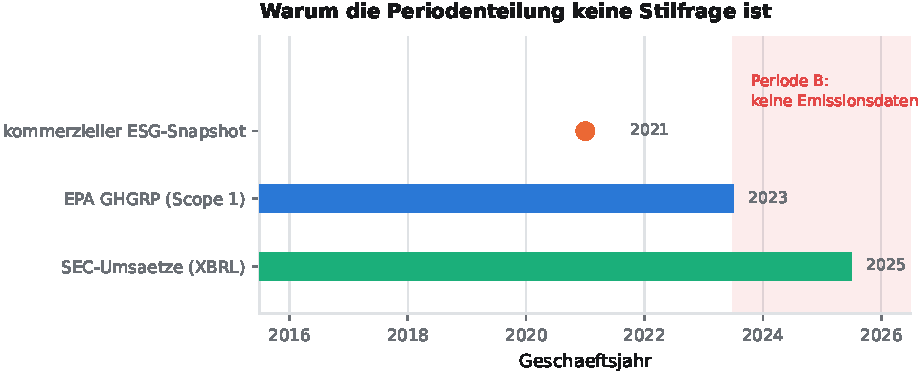
\includegraphics[width=0.86\textwidth]{figures/verfuegbarkeit.pdf}
\caption{Die Periodenteilung folgt der Datenlage, nicht einer Darstellungsentscheidung. Die Umsatzreihe läuft bis Geschäftsjahr 2025 weiter, die Emissionsreihe endet 2023.}
\label{fig:verfuegbarkeit}
\end{figure}

\textbf{Periode~A (Geschäftsjahre 2018--2023).} Alles vorhanden: Anlagenemissionen, Umsätze, dazu ein kommerzieller ESG-Snapshot als externer Vergleichsmaßstab. Hier lässt sich nicht nur ranken, sondern auch prüfen.

\textbf{Periode~B (ab Geschäftsjahr 2024).} Für das Berichtsjahr 2024 war die Meldefrist der 30.~Mai 2025. Die Daten sind eingereicht, aber bis heute nicht veröffentlicht -- weder über FLIGHT noch über Envirofacts. Für 488 der 503 Firmen liegt der Umsatz 2025 vor, für null Firmen die Emissionen. Das ist keine Qualitätsverschlechterung, sondern ein vollständiger Ausfall der wichtigsten Eingangsgröße.

\section{Periode A: Ergebnisse}

\subsection{Wer überhaupt bewertet werden kann}

\begin{figure}[htbp]
\centering
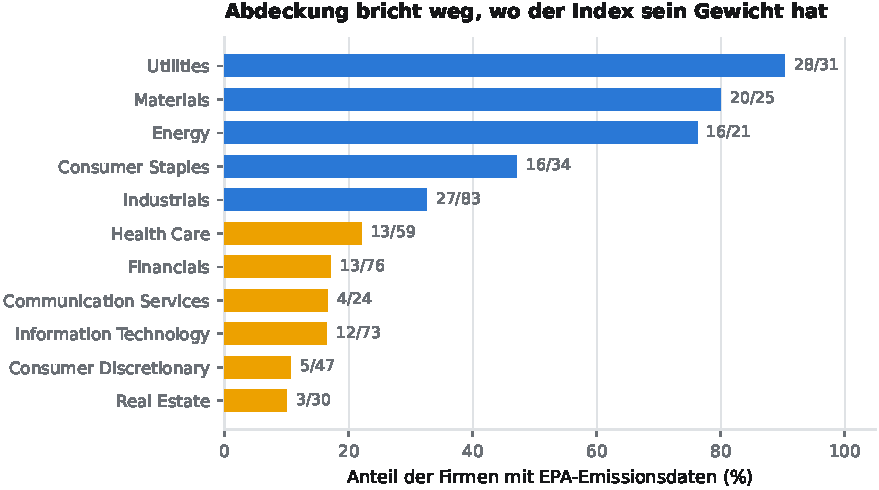
\includegraphics[width=0.92\textwidth]{figures/abdeckung_sektor.pdf}
\caption{Anteil der Indexmitglieder je GICS-Sektor, für die Emissionsdaten vorliegen. Die Lücke ist nicht zufällig verteilt.}
\label{fig:abdeckung}
\end{figure}

Bei den Versorgern sind 28 von 31 Firmen erfasst, bei Grundstoffen 20 von 25, in der Energiebranche 16 von 21. Am anderen Ende: Informationstechnologie 12 von 73, Finanzen 13 von 76, Immobilien 3 von 30.

\befund{\textbf{Das ist die wichtigste Einschränkung des ganzen Modells.} Die 157 bewertbaren Firmen sind keine Stichprobe des S\&P~500, sondern seine Schwerindustrie. Wer bei Microsoft, JPMorgan oder Visa nach Emissionen sucht, findet fast nichts -- nicht weil diese Firmen sauber wären, sondern weil ihr Fußabdruck in Scope~2 und Scope~3 liegt, wo es keine freien Daten gibt. Das Ranking beantwortet damit nicht die Frage \glqq wer ist nachhaltig\grqq, sondern \glqq wer betreibt große Schornsteine, und wie effizient\grqq.}

\subsection{Das Band ist das Ergebnis}

\begin{figure}[htbp]
\centering
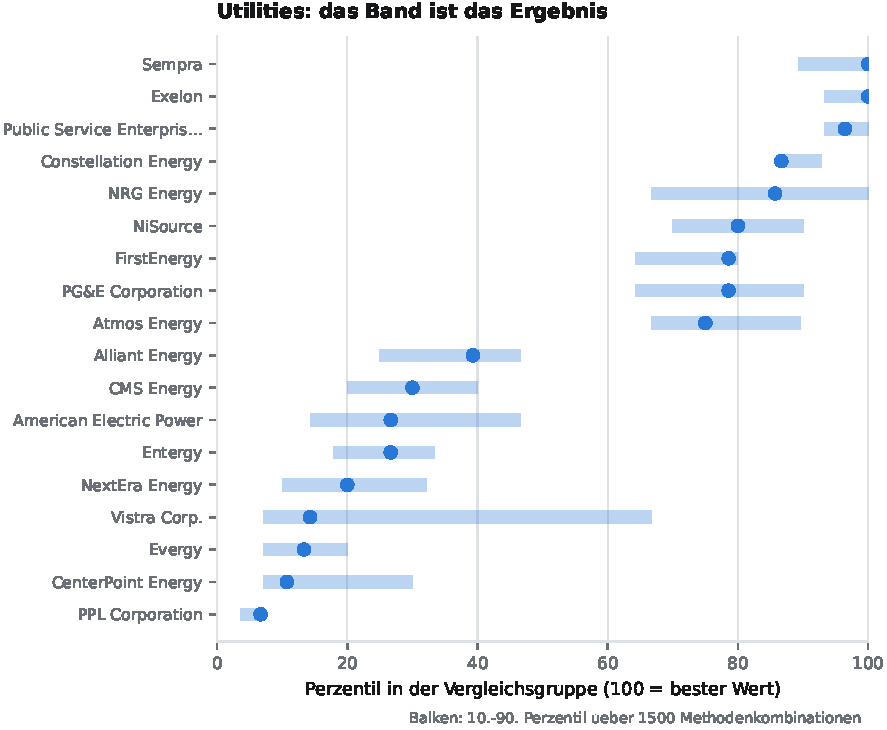
\includegraphics[width=0.9\textwidth]{figures/rangbaender.pdf}
\caption{Versorger, sortiert nach Median-Perzentil. Der Punkt ist der Median über 1500 Methodenkombinationen, der Balken das Intervall vom 10.\ bis zum 90.\ Perzentil.}
\label{fig:baender}
\end{figure}

Abbildung~\ref{fig:baender} zeigt, warum Einzelplätze irreführend sind. Vistra hat ein Band von 8 bis 66 -- je nach Methodenwahl liegt dieselbe Firma im schlechtesten Zehntel oder im oberen Mittelfeld. Bei PPL dagegen reicht das Band von 4 bis 7: diese Einordnung hält jeder Methode stand.

\begin{figure}[htbp]
\centering
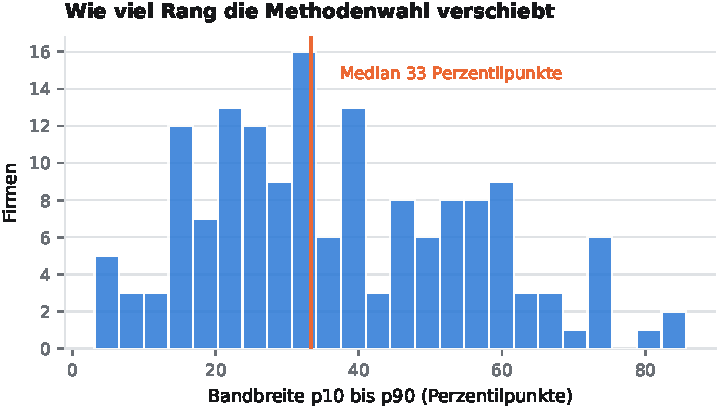
\includegraphics[width=0.9\textwidth]{figures/bandbreiten.pdf}
\caption{Verteilung der Bandbreiten über alle 157 bewerteten Firmen.}
\label{fig:bandbreiten}
\end{figure}

\subsection{Woher die Unsicherheit kommt}

Eine Bandbreite ist nur dann eine Aussage, wenn man weiß, woraus sie besteht. Deshalb wurde die Analyse dreimal gerechnet: einmal mit variierenden Methoden und abgeschaltetem Rauschen, einmal mit fester Referenzmethode und eingeschaltetem Rauschen, einmal mit beidem.

\begin{table}[htbp]
\centering\small
\caption{Zerlegung der Bandbreite (Median über alle Firmen, in Perzentilpunkten)}
\label{tab:zerlegung}
\begin{tabular}{lr}
\toprule
\textbf{Quelle der Unsicherheit} & \textbf{Median-Bandbreite} \\
\midrule
nur Methodenwahl (Rauschen aus) & 20{,}0 \\
nur Datenrauschen (Methode fest) & 15{,}0 \\
beides zusammen & 33{,}3 \\
\bottomrule
\end{tabular}
\end{table}

Die Methodenwahl trägt mehr bei als die Rauschannahme. Das ist beruhigend, weil es bedeutet, dass die Bandbreite kein Artefakt gesetzter Parameter ist. Es ist aber auch ein Ergebnis, das mit Vorsicht zu behandeln ist: die Rauschparameter sind gesetzt und nicht gemessen (siehe Schwachstelle~3).

Bei durchschnittlich 14{,}3 Firmen je Vergleichsgruppe entspricht ein Rangplatz rund 7 Perzentilpunkten. Die mediane Bandbreite von 33{,}3 Punkten sind damit \textbf{knapp fünf Rangplätze}.

\subsection{Welche Methodenentscheidung wie stark wirkt}

\begin{figure}[htbp]
\centering
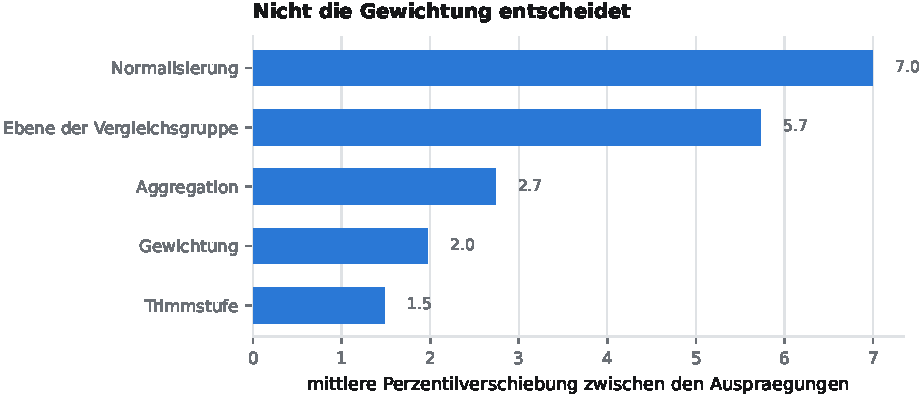
\includegraphics[width=0.9\textwidth]{figures/methoden_sensitivitaet.pdf}
\caption{Mittlere Perzentilverschiebung zwischen den Ausprägungen jeder Methodendimension.}
\label{fig:sensitivitaet}
\end{figure}

Die Reihenfolge ist bemerkenswert. Die Normalisierung -- also \emph{wie} gemessen wird -- verschiebt mit 7{,}0 Punkten am stärksten. Die Wahl der Vergleichsgruppe -- also \emph{was} verglichen wird -- folgt mit 5{,}7. Die Gewichtung liegt mit 2{,}0 fast am Ende.

\befund{\textbf{Ein empirisches Echo.} Die Literatur zerlegt die Uneinigkeit zwischen ESG-Anbietern in Messung (56\,\%), Umfang (38\,\%) und Gewichtung (6\,\%). Unsere Rangfolge reproduziert genau dieses Muster an einem völlig anderen Datensatz und mit nur drei Kennzahlen: Messverfahren zuerst, Abgrenzung zweitens, Gewichtung zuletzt. Wer eine Diskussion über Gewichte führt, diskutiert den kleinsten Hebel.}

\subsection{Geometrisch gegen additiv}
\label{sec:aggregation}

\begin{figure}[htbp]
\centering
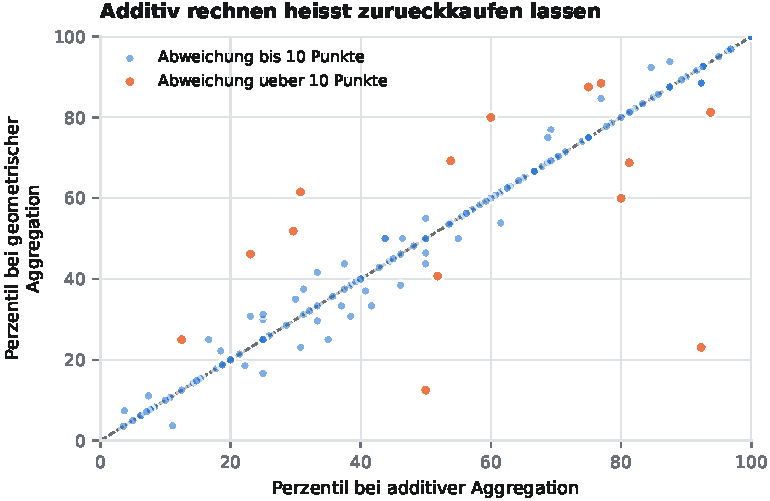
\includegraphics[width=0.86\textwidth]{figures/aggregation_vergleich.pdf}
\caption{Dieselben Firmen, einmal multiplikativ und einmal additiv zusammengefasst.}
\label{fig:aggregation}
\end{figure}

Das Ergebnis widerspricht der Erwartung. Die mediane absolute Abweichung zwischen beiden Verfahren beträgt \textbf{exakt null Perzentilpunkte}. Nur 8{,}9\,\% der Firmen verschieben sich um mehr als zehn Punkte, der Maximalwert liegt bei 69.

Der Grund steht in der Korrelationsmatrix: \texttt{intensity\_cagr} und \texttt{absolute\_cagr} korrelieren mit $\rho = 0{,}64$, weil beide aus derselben Emissionsreihe stammen. Effektiv liegen nur rund zwei unabhängige Dimensionen vor. Nicht-Kompensierbarkeit kann aber nur dort greifen, wo es tatsächlich etwas zu kompensieren gibt -- bei stark korrelierten Kennzahlen ist eine Firma in allen gleichzeitig gut oder schlecht.

\befund{\textbf{Die als entscheidend beschriebene Entscheidung entscheidet hier nichts.} Die multiplikative Aggregation ist methodisch richtig und bleibt die Voreinstellung. Mit dem aktuellen Kennzahl-Set ist sie aber weitgehend wirkungslos. Sie wird erst dann zur scharfen Klinge, wenn wirklich unabhängige Dimensionen vorliegen -- Governance, Wasser, Abfall. Genau die fehlen.}

\subsection{Vergleich mit einer gekauften Note}

\begin{figure}[htbp]
\centering
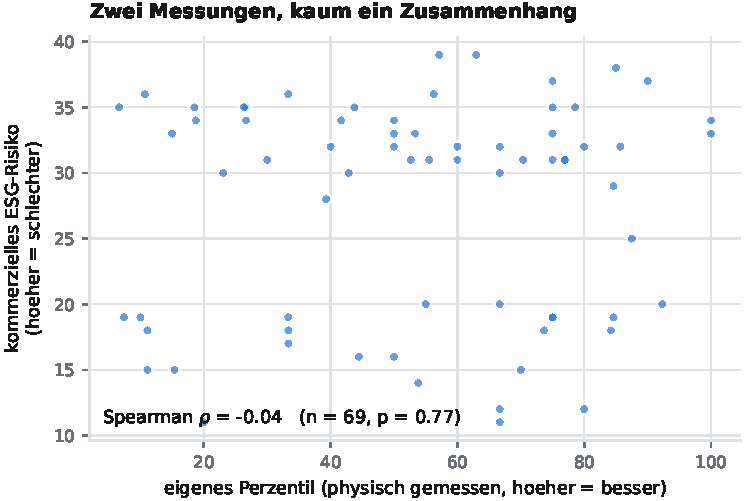
\includegraphics[width=0.86\textwidth]{figures/vergleich_kommerziell.pdf}
\caption{Das eigene, physisch gemessene Perzentil gegen ein kommerzielles ESG-Risikorating für die 69 Firmen, die in beiden Datensätzen vorkommen.}
\label{fig:kommerziell}
\end{figure}

Die Rangkorrelation beträgt $\rho = -0{,}04$ ($p = 0{,}77$). Für die reine Umweltkomponente des kommerziellen Ratings ergibt sich $\rho = 0{,}11$ ($p = 0{,}38$). In beiden Fällen: kein nachweisbarer Zusammenhang.

Aufgeschlüsselt nach Branche wird es deutlicher (Tabelle~\ref{tab:sektorkorr}): Das Vorzeichen kippt.

\begin{table}[htbp]
\centering\small
\caption{Rangkorrelation zwischen eigener und kommerzieller Bewertung, je Sektor}
\label{tab:sektorkorr}
\begin{tabular}{lrr}
\toprule
\textbf{Sektor} & \textbf{n} & \textbf{Spearman $\rho$} \\
\midrule
Materials & 8 & $-0{,}78$ \\
Information Technology & 9 & $-0{,}26$ \\
Consumer Staples & 6 & $0{,}03$ \\
Health Care & 6 & $0{,}03$ \\
Industrials & 11 & $0{,}07$ \\
Utilities & 13 & $0{,}51$ \\
\bottomrule
\end{tabular}
\end{table}

Bei den Versorgern besteht ein moderat positiver Zusammenhang -- dort misst die kommerzielle Note offenbar etwas Ähnliches. Bei den Grundstoffen ist er stark negativ: Firmen, die wir nach gemessenen Tonnen als gut einstufen, gelten dem Anbieter als schlecht, und umgekehrt.

\befund{\textbf{Vorsicht bei der Deutung.} Die Gruppen sind klein (n zwischen 6 und 13) und der Snapshot ist von 2021, unsere Werte von 2023. Der Befund taugt als Hinweis, nicht als Beweis. Er ist trotzdem unangenehm konkret: Man kann sich nicht darauf verlassen, dass eine gekaufte Note dasselbe misst wie eine gemessene -- nicht einmal im Vorzeichen.}

\subsection{Größen-Verzerrung}

\begin{figure}[htbp]
\centering
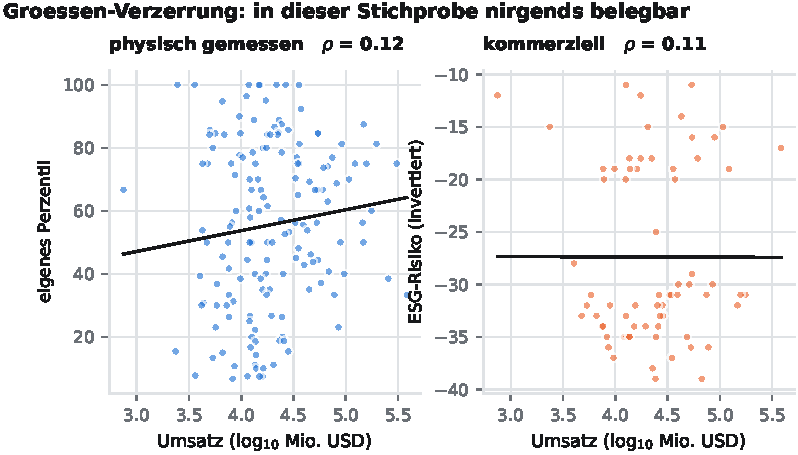
\includegraphics[width=0.95\textwidth]{figures/groessen_verzerrung.pdf}
\caption{Bewertung gegen Firmengröße, links physisch gemessen, rechts kommerziell.}
\label{fig:groesse}
\end{figure}

Die Literatur berichtet, dass große Firmen bessere ESG-Noten bekommen, weil sie sich eine Nachhaltigkeitsabteilung leisten können. In dieser Stichprobe lässt sich das nicht bestätigen: eigene Note $\rho = 0{,}12$ ($p = 0{,}12$, n = 157), kommerzielle Note $\rho = 0{,}11$ ($p = 0{,}36$, n = 69). Beide Werte sind klein und nicht signifikant.

Das ist ausdrücklich \emph{kein} Gegenbeweis zur Literatur. Bei n = 69 hat der Test schlicht nicht genug Kraft, um einen Effekt dieser Größenordnung nachzuweisen.

\subsection{Achse B: Greenwashing-Signale}

\begin{figure}[htbp]
\centering
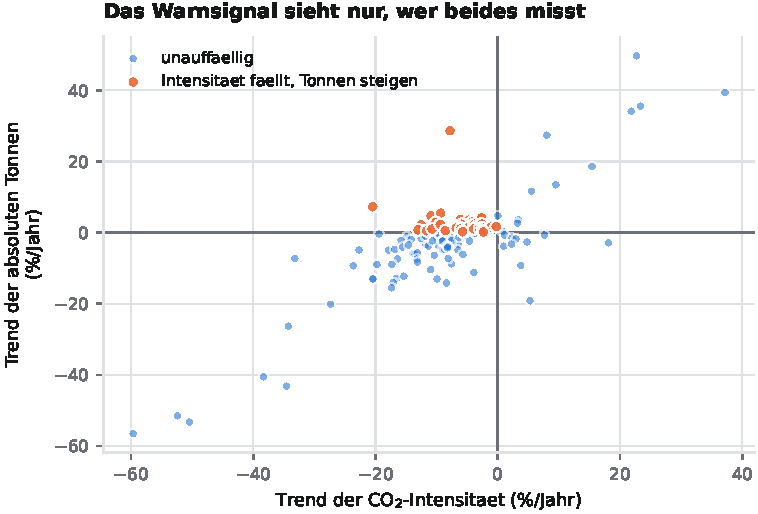
\includegraphics[width=0.86\textwidth]{figures/greenwashing_achse.pdf}
\caption{Trend der Intensität gegen Trend der absoluten Tonnen. Im Quadranten rechts unten von der Mitte liegt das Warnsignal: die Intensität fällt, der Ausstoß steigt.}
\label{fig:greenwashing}
\end{figure}

Zwei der sechs bekannten Warnsignale lassen sich aus den vorhandenen Daten berechnen:

\begin{itemize}
\item \textbf{Intensitäts-Illusion} (35 Firmen). Die CO\textsubscript{2}-Intensität sinkt, die absoluten Tonnen steigen. Das Musterbeispiel ist Tesla: Intensität $-7{,}8\,\%$ pro Jahr bei absolut $+28{,}6\,\%$ pro Jahr. Beides stimmt, beides lässt sich berichten -- nur eines davon reduziert Emissionen.
\item \textbf{Bequemes Basisjahr} (48 Firmen). Das erste Jahr des Betrachtungsfensters liegt mehr als 10\,\% über dem Median der Reihe. Jede spätere Reduktion sieht dann beeindruckender aus, als sie ist.
\end{itemize}

82 der 157 Firmen (52{,}2\,\%) zeigen mindestens ein Signal, eine Firma beide. Zum Vergleich: Die Literatur findet bei 4131 Firmen mit Klimaversprechen 96\,\% mit mindestens einem Warnsignal -- allerdings über alle sechs Signale. Mit einem Drittel der Signale erreichen wir gut die Hälfte des Anteils, was größenordnungsmäßig zusammenpasst.

Diese Werte fließen nicht in die Kernnote ein und werden getrennt ausgewiesen. Eine Firma kann sauber wirtschaften und unglaubwürdig berichten -- das sind zwei verschiedene Informationen.

\section{Periode B: was nach 2023 übrig bleibt}

\subsection{Der Befund}

Für Geschäftsjahre ab 2024 gibt es keine freien Emissionsdaten auf Firmenebene. Climate TRACE liefert zwar aktuellere Jahre, aber ohne Eigentümerzuordnung; die SBTi-Liste hat kein API; die EPA hat nicht veröffentlicht. Was bleibt, sind Umsätze für 488 Firmen -- der Nenner ohne Zähler.

\subsection{Was eine Fortschreibung kostet}

Die praktische Frage lautet nicht, ob das ideal ist, sondern ob eine Fortschreibung alter Emissionsdaten noch etwas Brauchbares ergibt. Das lässt sich rückwärts messen: Emissionen aus 2021 mit Umsätzen aus 2023 kombinieren und gegen die echte Rangliste 2023 halten.

\begin{figure}[htbp]
\centering
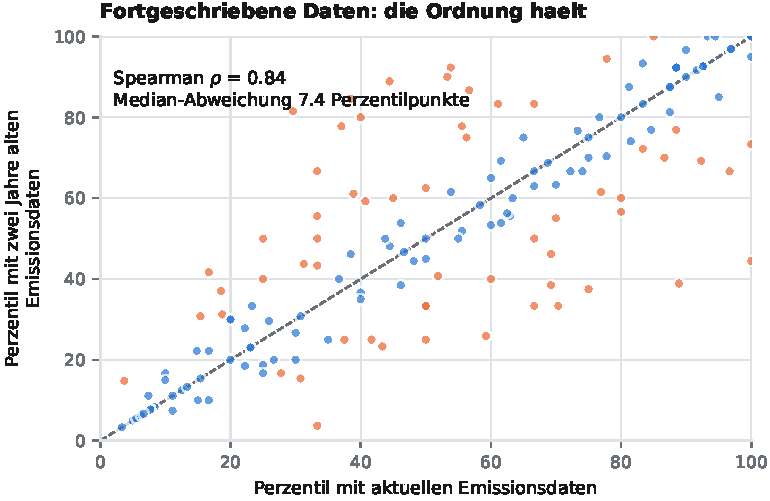
\includegraphics[width=0.86\textwidth]{figures/staleness_backtest.pdf}
\caption{Rückwärtstest über 161 Firmen. Orange markiert sind Firmen, die sich um mehr als zehn Perzentilpunkte verschieben.}
\label{fig:staleness}
\end{figure}

\begin{table}[htbp]
\centering\small
\caption{Kosten einer zweijährigen Fortschreibung}
\label{tab:staleness}
\begin{tabular}{lr}
\toprule
Rangkorrelation zur echten Rangliste & $\rho = 0{,}84$ \\
Median-Abweichung & 7{,}4 Perzentilpunkte \\
90.\ Perzentil der Abweichung & 30{,}0 Perzentilpunkte \\
Anteil der Firmen mit über 10 Punkten Abweichung & 37{,}3\,\% \\
\bottomrule
\end{tabular}
\end{table}

\befund{\textbf{Die Antwort ist ein bedingtes Ja.} Die grobe Ordnung bleibt erhalten -- wer unten steht, steht auch mit alten Daten unten. Aber gut ein Drittel der Firmen verschiebt sich um mehr als einen Rangplatz, und das oberste Zehntel der Abweichungen liegt bei 30 Perzentilpunkten, also mehr als vier Rangplätzen. Eine Fortschreibung ist vertretbar, wenn das Band um diesen gemessenen Fehler aufgeweitet wird und das Datenalter je Firma angezeigt wird. Sie ist nicht vertretbar, wenn das Ergebnis so präsentiert wird wie in Periode~A.}

\section{Schwachstellen des Ansatzes}
\label{sec:schwach}

Die folgenden zehn Punkte sind am Modell gemessen, nicht vermutet.

\paragraph{1. Die Abdeckung ist strukturell verzerrt, nicht nur lückenhaft.}
157 von 503 Firmen. Entscheidend ist nicht die Zahl, sondern das Muster: Versorger 90\,\%, Immobilien 10\,\%. Die fehlenden Firmen fehlen systematisch, weil ihre Emissionen in Scope~2 und~3 liegen. Das Modell misst damit eine andere Frage als die, die es zu beantworten vorgibt.

\paragraph{2. Der GICS-Sektor ist die falsche Vergleichsgruppe.}
Berkshire Hathaway steht mit 53{,}7~Mio.~\tco{} unter \emph{Financials} und wird gegen Banken verglichen. Das Ergebnis sagt nichts über das Verhalten der Firma, sondern nur über die Willkür einer Branchentaxonomie, die nach Umsatzquellen sortiert und nicht nach Emissionsprofil. Die feinere Ebene ist keine Lösung: Die Sub-Industry-Gruppen haben eine Mediangröße von genau einer Firma.

\paragraph{3. Die Rauschparameter sind gesetzt, nicht gemessen.}
Die Unsicherheitsanalyse verwendet ein Grundrauschen von 5\,\% der Querschnittsstreuung plus bis zu 35\,\% für unsicher zugeordnete Firmen. Beide Zahlen sind plausibel gewählt und durch nichts belegt. Damit ist ein knappes Drittel der ausgewiesenen Bandbreite eine Annahme, die als Messung aussieht.

\paragraph{4. Drei Kennzahlen sind zu wenig, und zwei messen fast dasselbe.}
$\rho = 0{,}64$ zwischen den beiden Trendkennzahlen. Effektiv bleiben zwei Dimensionen. Die Folge ist in Abschnitt~\ref{sec:aggregation} gemessen: die multiplikative Aggregation, methodisch das Herzstück, verändert im Median nichts.

\paragraph{5. Kleine Gruppen machen Perzentile grobkörnig.}
Immobilien n = 3, Communication Services n = 4, Consumer Discretionary n = 5. In einer Dreiergruppe entspricht ein Rangplatz 33 Perzentilpunkten. Die Bänder dieser Firmen sind Artefakte der Gruppengröße und keine Aussage über Unsicherheit.

\paragraph{6. Die Greenwashing-Achse hat zwei von sechs Signalen.}
Es fehlen ausgerechnet die aussagekräftigsten: fehlende Zwischenziele, Scope-3-Abdeckung, Kompensations\-abhängigkeit und widersprüchliche Lobbyarbeit. Das stärkste Einzelsignal überhaupt -- die Lücke zwischen versprochenem und tatsächlichem Reduktionspfad -- ist ohne SBTi-Daten nicht berechenbar.

\paragraph{7. Der Basisjahr-Indikator misst das falsche Basisjahr.}
Er prüft, ob das erste Jahr \emph{unseres Fensters} ungewöhnlich hoch liegt. Relevant wäre das Jahr, das die Firma in ihrem eigenen Versprechen als Basis beansprucht. Ohne Zieldaten ist der Indikator ein Näherungswert mit unbekannter Trefferquote.

\paragraph{8. Der Vergleichsmaßstab ist zwei Jahre älter als die Bewertung.}
Der ESG-Snapshot hat den Stand 2021, die Rangliste bezieht sich auf 2023. Der Befund $\rho = -0{,}04$ vermischt echte Uneinigkeit mit zeitlicher Verschiebung. Er ist damit ein Hinweis, kein Nachweis.

\paragraph{9. Die Zurechnungsregel ist eine Wahl unter mehreren.}
Verwendet wird der Equity-Share-Ansatz. Das GHG-Protokoll kennt daneben die Kontrollansätze, bei denen der Betreiber einer Anlage 100\,\% übernimmt statt seines Anteils. Bei einer 50/50-Anlage unterscheiden sich die Ergebnisse um den Faktor zwei. Diese Wahl steckt derzeit fest im Code, statt als Dimension in der Unsicherheitsanalyse zu erscheinen.

\paragraph{10. Überlebensverzerrung in der Indexliste.}
Für die Jahre 2018--2023 wird die \emph{heutige} S\&P-500-Zusammensetzung verwendet. Firmen, die seither aus dem Index geflogen sind, fehlen vollständig -- und das sind tendenziell die schlechter laufenden. Der historische Teil der Auswertung ist dadurch nach oben verzerrt.

\section{Verbesserungsvorschläge}
\label{sec:verbesser}

Sortiert nach Verhältnis von Wirkung zu Aufwand.

\paragraph{V1 -- Zwei getrennte Listen statt einer (Aufwand: Stunden).}
Statt eine \glqq S\&P-500-Rangliste\grqq{} zu behaupten, zwei Ausgaben liefern: eine anlagenbasierte Rangliste für die rund 91 Firmen aus Versorgern, Energie, Grundstoffen und Industrie, wo die Datengrundlage trägt -- und eine ausdrückliche Liste \glqq nicht bewertbar\grqq{} mit Begründung je Firma. Das ist keine Einschränkung des Produkts, sondern die einzige ehrliche Form davon. Zusätzlich je Firma die Abdeckungsquote als sichtbare Kennzahl anzeigen.

\paragraph{V2 -- Vergleichsgruppen aus den Daten bilden (Aufwand: ein Tag).}
Statt GICS eine Gruppierung nach Emissionsprofil: k-Means über die NAICS-Anteile der zugeordneten Anlagen, mit erzwungener Mindestgröße von acht. Berkshire Hathaway landet dann bei den Versorgern, wo es nach seinem Emissionsprofil hingehört, und nicht bei den Banken. Die Sektorzuordnung bleibt als zweite Sicht erhalten, damit der Vergleich mit externen Ratings möglich bleibt.

\paragraph{V3 -- Unsicherheit messen statt setzen (Aufwand: ein Tag).}
Die EPA liefert im Feld \texttt{cems\_used} die Angabe, ob eine Anlage kontinuierlich gemessen oder geschätzt meldet. Daraus lässt sich eine datengestützte Unsicherheit je Anlage ableiten, statt einen Pauschalwert zu setzen. Für die Zuordnungsunsicherheit dasselbe Prinzip: die Rangliste über mehrere Matching-Schwellen (85, 90, 92, 95) rechnen und die resultierende Streuung als empirisches Rauschen verwenden. Damit wird die Bandbreite zu einer Messung.

\paragraph{V4 -- Kennzahl-Set entkoppeln (Aufwand: ein bis zwei Tage).}
Die beiden korrelierten Trends durch unabhängigere Größen ersetzen oder ergänzen:
\begin{itemize}
\item \emph{Trendabweichung zur Branche} statt absolutem Trend -- misst, ob eine Firma schneller sinkt als ihre direkte Konkurrenz, und ist damit unabhängig vom Niveau.
\item \emph{Emissionskonzentration} (Herfindahl-Index über die Anlagen einer Firma) -- eine Firma mit drei Großanlagen kann anders umbauen als eine mit 140 kleinen. Diese Größe ist aus den vorhandenen Daten sofort berechenbar und mit nichts anderem korreliert.
\item \emph{Anteil der Emissionen aus CEMS-gemessenen Anlagen} -- misst Messqualität und damit Berichtsernsthaftigkeit.
\end{itemize}
Erst mit unabhängigen Dimensionen wird die geometrische Aggregation zu dem Instrument, als das sie gedacht ist.

\paragraph{V5 -- SBTi-Daten einmalig abziehen (Aufwand: zwei bis drei Stunden).}
Das Target-Dashboard hat kein öffentliches API, lädt seine Tabelle aber über einen internen Endpunkt nach. Diesen einmal per Headless-Browser mitschneiden, das Ergebnis als CSV mit Abrufdatum einfrieren und als reguläre Quelle registrieren. Das schließt die größte Lücke der Achse~B und macht die Kennzahl \glqq Lücke zwischen Versprechen und Realität\grqq{} überhaupt erst berechenbar -- das stärkste bekannte Einzelsignal.

\paragraph{V6 -- Fortschreibung mit gemessenem Warnband (Aufwand: Stunden).}
Für Periode~B die Fortschreibung erlauben, aber das Band um den im Rückwärtstest gemessenen Fehler aufweiten und das Datenalter je Firma anzeigen. Konkret: Bandbreite $+30$ Perzentilpunkte im ungünstigen Fall, Kennzeichnung \glqq Emissionsdaten von 2023\grqq. Zusätzlich prüfen, ob eine Skalierung mit dem Climate-TRACE-Sektortrend die Fortschreibung verbessert -- das ist mit demselben Rückwärtstest messbar und entweder eine Verbesserung oder ein dokumentierter Fehlschlag.

\paragraph{V7 -- Zurechnungsregel als Unsicherheitsdimension (Aufwand: eine Stunde).}
Equity-Share und operative Kontrolle beide implementieren und als weitere Achse in den Kombinationsraum aufnehmen. Zwanzig Zeilen Code, die eine bisher versteckte Ermessensentscheidung sichtbar machen.

\paragraph{V8 -- Indexhistorie rekonstruieren (Aufwand: ein halber Tag).}
Die Änderungsliste der Indexzusammensetzung ist frei verfügbar. Damit lässt sich für jedes Jahr die damals gültige Mitgliederliste herstellen und die Überlebensverzerrung beseitigen.

\paragraph{V9 -- Stichprobenvalidierung gegen Selbstauskunft (Aufwand: ein halber Tag).}
Ein Teil der Firmen berichtet Scope~1 im eigenen Nachhaltigkeitsbericht. Zwanzig Firmen von Hand gegen unsere aus Anlagendaten aufsummierten Werte halten. Das ist die einzige direkte Prüfung, ob die Entity Resolution funktioniert -- alles andere ist Plausibilität. Erwartbare Abweichungen: unsere Werte liegen systematisch niedriger, weil Anlagen unter der Meldeschwelle von 25\,000~t und alle Auslandsanlagen fehlen. Die Größenordnung dieser Lücke zu kennen, ist wertvoller als jede weitere Methodenvariante.

\section{Reproduktion}

\begin{table}[htbp]
\centering\small
\caption{Ablauf}
\label{tab:repro}
\begin{tabular}{ll}
\toprule
\texttt{python scripts/01\_fetch.py} & alle Quellen ziehen, als Parquet cachen \\
\texttt{python scripts/02\_analyse.py} & Zuordnung, Monte Carlo, beide Perioden \\
\texttt{python scripts/03\_grafiken.py} & Grafiken erzeugen \\
\bottomrule
\end{tabular}
\end{table}

Der Monte-Carlo-Lauf verwendet 1500 Züge aus einem Kombinationsraum von 576 Methodenkombinationen (4 Normalisierungen $\times$ 3 Gewichtungen $\times$ 2 Aggregationen $\times$ 2 Gruppenebenen $\times$ 3 Trimmstufen $\times$ 4 Kennzahl-Teilmengen). Der Zufallsstartwert ist fest gesetzt, die Ergebnisse sind damit exakt wiederholbar. Laufzeit der vollständigen Auswertung: 87 Sekunden.

Alle Zwischenergebnisse liegen als CSV in \texttt{data/out}: die Firma-Jahr-Tabelle, die Rangbänder, die Greenwashing-Achse, die Abdeckung je Sektor, der Aggregationsvergleich, die Methodensensitivität und der Rückwärtstest. Die Datei \texttt{kennzahlen.json} enthält alle im Bericht zitierten Werte.

\vfill
\befund{\textbf{Was dieser Bericht nicht behauptet.} Er stellt nicht fest, dass eine bestimmte Firma täuscht. Er behauptet keine Aussage über Firmen ohne Anlagendaten. Er misst Scope~1 und nennt das ausdrücklich eine Eingrenzung, keine Vollständigkeit. Und er gibt keine Rangplätze aus, wo die Daten nur Bänder hergeben.}

\end{document}
